\section{Results}
\label{results}

The conversion counting in a given volume can be translated into a material budget estimate once the efficiency and the impinging 
photon flux are correctly taken into account. 
In particular, assuming a negligible background, the number of reconstructed photon conversion $N_{\rm reco}$ in a given volume bin is
\begin{equation}
N_{\rm reco} \propto \varepsilon \cdot \langle \frac{P}{X_0} \rangle \cdot f_{\rm geom}
\end{equation}
where $\varepsilon$ is the reconstruction efficiency and $\langle P/{X_0} \rangle$ is the average conversion probability ($P\sim 7/9$).

The present statistics allow only the pixel barrel to be studied. 
It is identified by choosing the following fiducial volume: $|z|<26~{\rm cm}$ and $r$ comprised between $0.8$ and $18\cm$.
Such region is divided for convenience into four parts corresponding to the beam pipe and the three pixel barrel layers, as detailed in Table~\ref{table:bins}.


\begin{table}[h]
\begin{center}
  \begin{tabular}{rccc}
    Label & $r_{\rm min}$ [$\cm$] & $r_{\rm max}$ [$\cm$] & Efficiency \\  
\hline
BP & 0.8 & 3.2 & 2.7\% \\
PXL1 & 3.2 & 6.0   & 3.5\% \\
PXL2 & 6.0 & 8.8 & 0.5\% \\
PXL3 & 8.8 & 18.0  & 0.1\% \\
  \end{tabular}
  \caption{Parameters and conversion reconstruction efficiency of the four regions of the pixel barrel volume corresponding to the beam pipe and the three pixel barrel layers, respectively.}
\label{table:bins}
\end{center}
\end{table}


%$1~{\rm cm}<r_{\rm BP}<3.5~{\rm cm}<r_{\rm PXL1}<6~{\rm cm}<r_{\rm PXL2}<8.4~{\rm cm}<r_{\rm PXL3}<15~{\rm cm}$. \\

The conversion finding efficiency $\varepsilon$, estimated from MC data for each sub-region, is also reported in Table~\ref{table:bins}.
%%2.8\%, 3.5\%, 0.5\% and 0.1\% respectively.

Figure~\ref{figMBvsr} represents an uncalibrated estimation, given in arbitrary units, 
comparing the material budget of the beam pipe and of the pixel barrel layers as a function of the radius $r$. The bin width is $0.2\cm$.
The correction factor $f^{r, z}_{\rm geom}$ is given by Eq.~\ref{eq:13}.
The green line shows the case of ideal resolution and efficiency, corrected for $f^{r, z}_{\rm geom}$.
Blue boxes represent MC pseudo data and black dots data; they are both corrected for $\varepsilon$ and $f^{r, z}_{\rm geom}$.
The conversion radius in data is computed with respect to the pixel center $(-0.1475\cm, -0.3782\cm, -0.4847\cm)$, 
as estimated from tracker alignment algorithms. 
The expected fake contribution, shown in red boxes, is not subtracted. 
Data show a good agreement with MC, both in shapes and in the overall number of entries.

\begin{figure}[!htbp]
 \begin{center}
   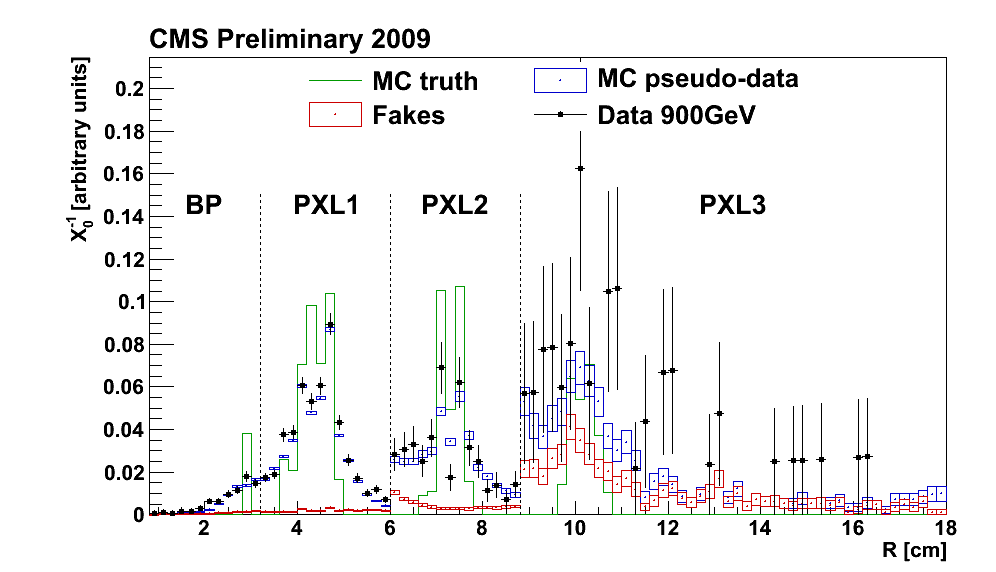
\includegraphics[width=\textwidth]{rPlot.png}
 \end{center}
 \caption{Uncalibrated material budget vs. radius; bin width equal to $0.2\cm$.}
\label{figMBvsr}
\end{figure}

Statistical fluctuations dominates the region of the third pixel layer in Fig.~\ref{figMBvsr}. The same plot done with a bin width of $0.4\cm$, shown in Fig.~\ref{figMBvsr_coarse}, allows a better reading of the third pixel layer region that is anyhow characterised by a large background contribution. 

\begin{figure}[!htbp]
 \begin{center}
   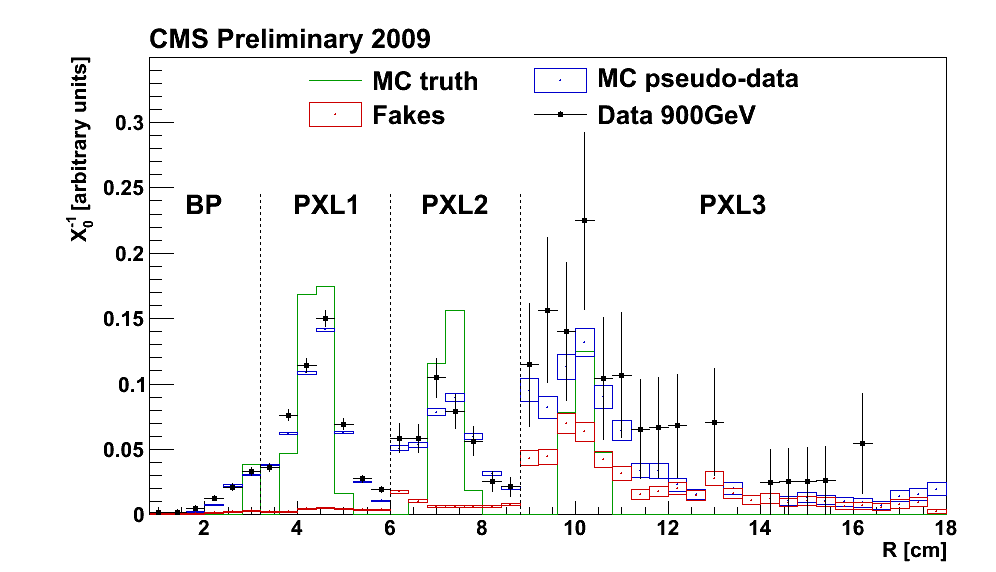
\includegraphics[width=\textwidth]{rPlot_coarse.png}
 \end{center}
 \caption{Uncalibrated material budget vs. radius; bin width equal to $0.4\cm$.}
\label{figMBvsr_coarse}
\end{figure}


Figure~\ref{xyPlot} and Figure~\ref{zrPlot} show the comparison in the $x$$-$$y$ and $z$$-$$r$ planes respectively, where the grey density 
gives an estimate of the amount of material in bins of size $0.25\cm\times0.25\cm$. 
The material in the $x$$-$$y$ plane is computed using the correction factor $f^{x, y}_{\rm geom}$ defined in Eq.~\ref{eq:15}.
The low statistics of reconstructed photon conversions does not allow a quantitative comparison of the results from data yet.

\begin{figure}[!hbtp]
\centering
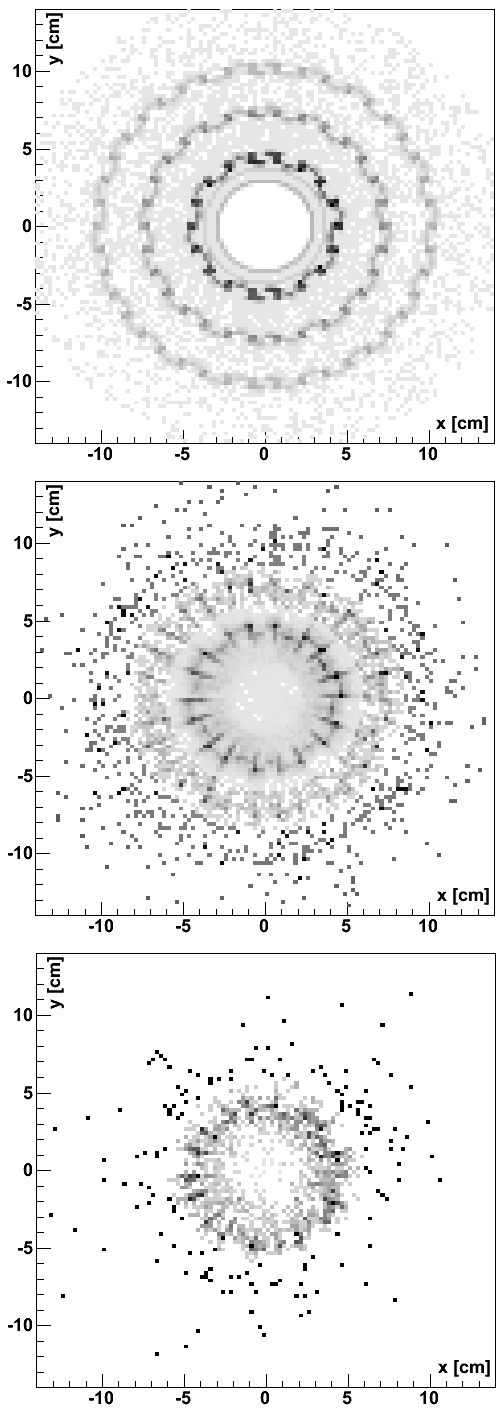
\includegraphics[height=0.9\textheight]{xyPlotVert.png}
\caption{Material budget estimation $x$$-$$y$ map. Top: MC truth; Center: MC pseudo-data; Bottom: data.}
\label{xyPlot}
\end{figure}

\begin{figure}[!hbtp]
\centering
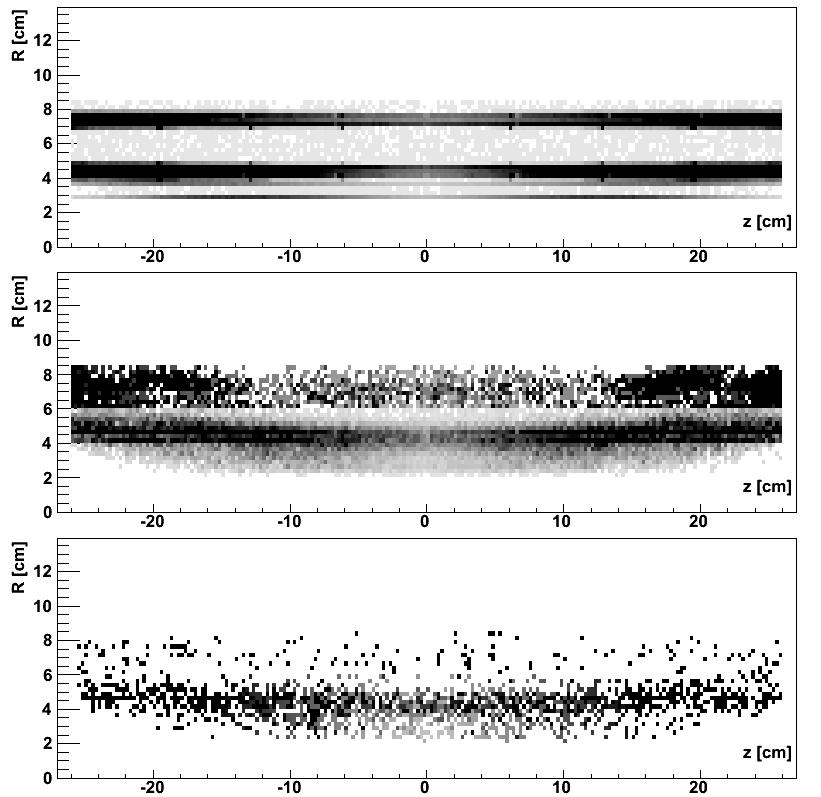
\includegraphics[width=\textwidth]{zrPlot.png}
\caption{Material budget estimation $z$$-$$r$ map. Top: MC truth; Center: MC pseudo-data; Bottom: data.}
\label{zrPlot}
\end{figure}
